%% ------------------------------------------------------------------------- %%
\section{Modelo do sinal}
\label{sec:modelo}

Uma onda sonora é uma vibração que se propaga em um meio físico, como o ar ou a água. O ouvido humano percebe tais vibrações como som e é capaz de ouvir frequências de aproximadamente 20Hz a 20kHz.

Para processarmos um sinal sonoro utilizando um computador digital, precisamos fazer uma amostragem desse sinal. A amostragem é feita a uma taxa R, chamada taxa de amostragem. Segundo o Teorema da amostragem de Nyquist–Shannon, a amostragem com precisão infinita, isto é, sem quantização de amplitude, contém toda a informação do sinal original, supondo que tal sinal seja limitado em uma banda de até R/2 Hz.

\begin{figure}[h]
\centering
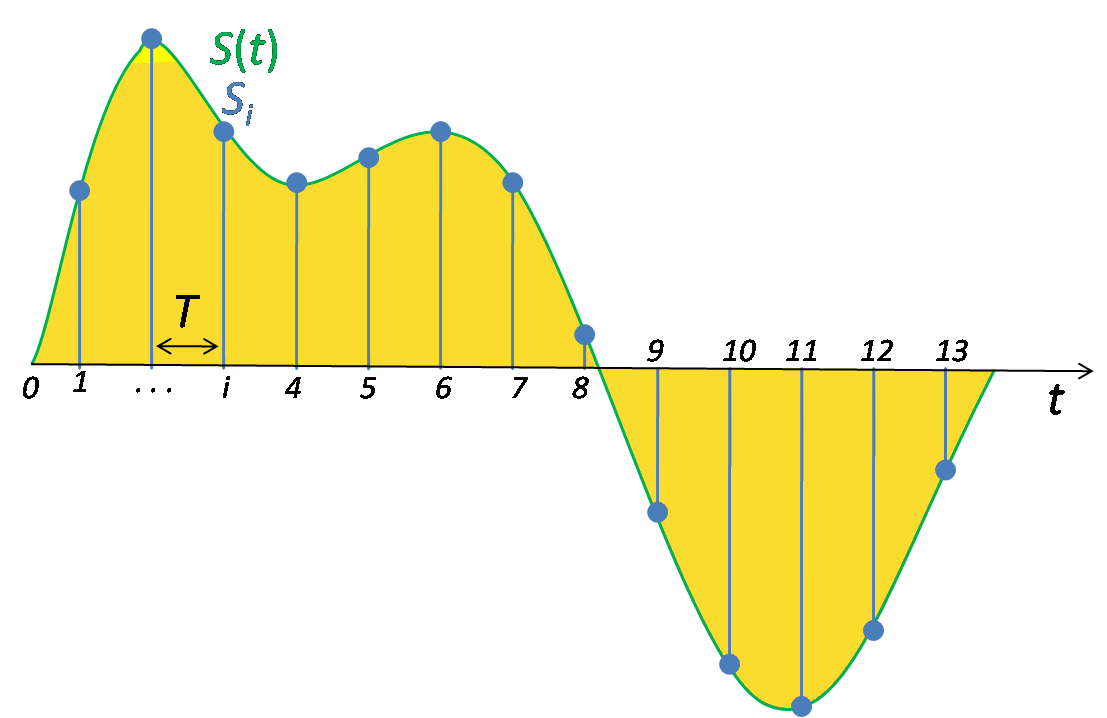
\includegraphics[width=0.6\linewidth]{figuras/Signal_Sampling.png}
\caption{\label{fig:Signal_Sampling}Demonstração de amostragem utilizada em processamento de sinais.}
\end{figure}

Um sinal digital é um sinal onde tanto o tempo quanto a amplitude são discretizados.

